\documentclass[a4paper]{article}

\usepackage{amsmath}
\usepackage{amssymb}
\usepackage{parskip}
\usepackage{fullpage}
\usepackage{hyperref}
\usepackage{bettelini}
\usepackage{graphicx}
\usepackage[backend=bibtex]{biblatex}

\hypersetup{
    colorlinks=true,
    linkcolor=black,
    urlcolor=blue,
    pdftitle={Chemistry},
    pdfpagemode=FullScreen,
}

\addbibresource{./references.bib}

\title{Chimica}
\author{Paolo Bettelini}
\date{}

\begin{document}

\maketitle
\tableofcontents

% 978.88.08.72527.1
% CHIMICA.BLU J.Brady

\pagebreak

\section{Chimica}

Sistema \(\subseteq\) Ambiente \(\subseteq\) Universo.

Un sistema può essere:
\begin{itemize}
    \item \textbf{Aperto:} se scambia materia/energia con l'ambiente.
    \item \textbf{Chiuso:} se scambia solo energia con l'ambiente.
    \item \textbf{Isolato:} se non scambia nè energia nè material con l'ambiente.
\end{itemize}

Studiare un sistema significa descrivere le sue proprietà
\begin{itemize}
    \item \textbf{Qualitative:} possono essere definite senza avvalersi
    di misure.
    \item \textbf{Quantitative:} richiedono delle misure.
\end{itemize}
Le priorità misurabili sono delle \textit{grandezze}.

% TODO intensive / estensive

\subsection{Notazione scientifica}

La notazione scientifica viene espressa come
\[
    a \cdot 10^k,\quad a\in [1, 10)
\]

\subsection{Sistema Internazionale}

\subsubsection{Grandezze fondamentali}

\begin{figure}[h]
    \centering
    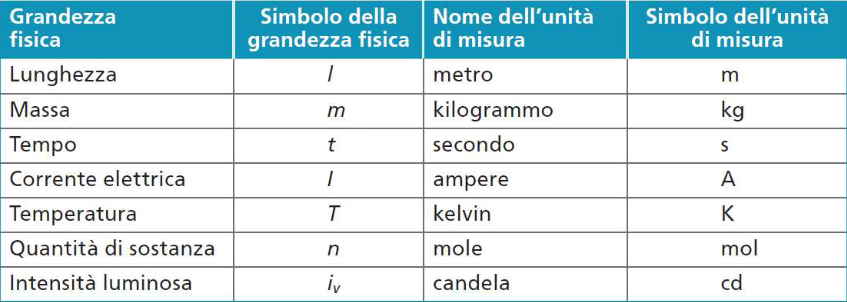
\includegraphics[width=0.75\textwidth]{./si.png}
\end{figure}

\subsubsection{Grandezze derivate}

\begin{figure}[h]
    \centering
    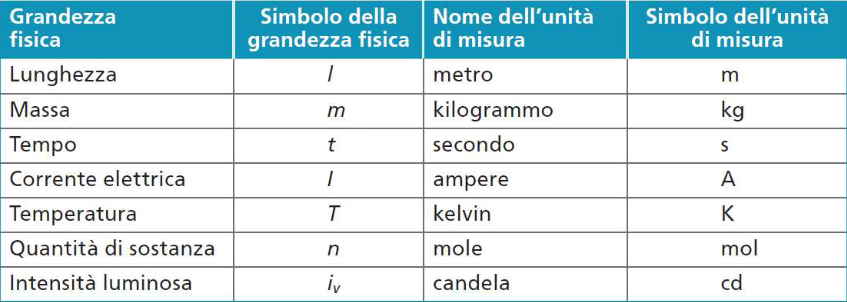
\includegraphics[width=0.75\textwidth]{./si.png}
\end{figure}

\pagebreak

\subsubsection{Misure}

\begin{figure}[h]
    \centering
    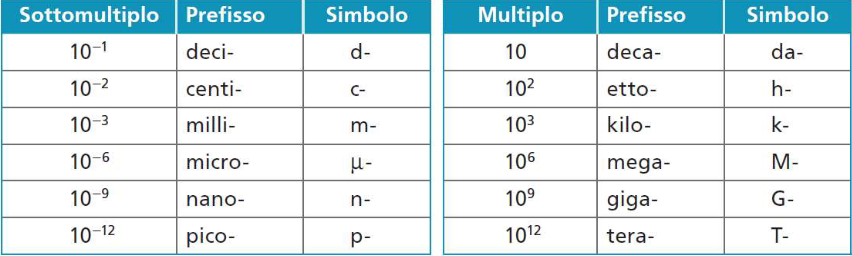
\includegraphics[width=0.75\textwidth]{./misure.png}
\end{figure}

\pagebreak

\section{Isotopi dell'idrogeno}

\subsection{Deuterio}

Il primo isotopo dell'idrogeno è il \textit{deuterio}, indicato con \(D\) o \(^2H\).
A differenza dell'idrogeno comune, il deuterio possiede un neutrone nel nucleo oltre al protone.
A causa di questa caratteristica, il deuterio ha una massa atomica leggermente superiore rispetto all'idrogeno normale.
Il deuterio è utilizzato in varie applicazioni, come nei reattori nucleari per la produzione di energia e come tracciatore in studi scientifici e biologici. 

\subsection{Trizio}

Il secondo isotopo dell'idrogeno è è il trizio, indicato con \(T\) o \(^3H\).
A differenza dell'idrogeno comune, il deuterio possiede due neutroni nel nucleo oltre al protone.
A causa di questa composizione nucleare, il trizio ha una massa atomica maggiore rispetto agli altri isotopi dell'idrogeno.
Il trizio è radioattivo e decade nel tempo con una emivita di circa 12,3 anni, emettendo particelle beta.

\section{Acqua con deuterio e trizio}

È possibile ottenere dell'acqua, \(H_2O\), utilizzando gli isotopi \(D\) e \(T\) al posto di \(H\).

Queste sostanze sono chiamate \textit{acqua pesante} (\(D_2O\)) e
\textit{acqua superpesante} (\(T_2O\)).

\subsection{Densità}

\begin{center}
    \bgroup{}
    \def\arraystretch{1.25}
    \begin{tabular}{ |c|c|c|c| }
        \hline
        & \textbf{Acqua} & \textbf{Acqua pesante} & \textbf{Acqua Superpesante} \\
        \hline
        \textbf{Liquido (g/cm\(^3\))} & 0.997 & 1.11 & 1.20 \\
        \hline
        \textbf{Solido (g/cm\(^3\))} & 0.9168 & 1.105 & ? \\
        \hline
    \end{tabular}
    \egroup{}
\end{center}

Normalmente, le molecole dell'acqua che ghiaccia si organizzano, e creano molti spazi (caso unico).
Questo implica che il ghiaccio abbia una densità minore dell'acqua, per cui esso galleggia se immerso nell'acqua.

Possiamo quindi notare dalla tabella come la versione solida dell'acqua pesante galleggi
nell'acqua normale \cite{deuterated-water}.

\nocite{*} % cite all entries

\printbibliography

\end{document}
